\documentclass[tikz,border=10pt]{standalone}
\usepackage{tikz}
\usepackage{amsmath}

\begin{document}

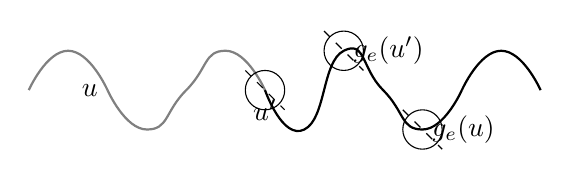
\begin{tikzpicture}
    % Original walk (gray)
    \draw[thick, gray] plot [smooth, tension=1] coordinates {(-2,0) (-1.5,-0.5) (-1,0) (-0.5,0.5) (0,0)};
    
    % Modified walk (black)
    \draw[thick] plot [smooth, tension=1] coordinates {(0,0) (0.5,-0.5) (1,0.5) (1.5,0) (2,-0.5) (2.5,0)};
    
    % Extensions
    \draw[thick, gray] plot [smooth, tension=1] coordinates {(-2,0) (-2.5,0.5) (-3,0)};
    \draw[thick] plot [smooth, tension=1] coordinates {(2.5,0) (3,0.5) (3.5,0)};
    
    % Splitting point and circles
    \node[circle, draw, minimum size=0.5cm] at (0,0) {};
    \node[circle, draw, minimum size=0.5cm] at (1,0.5) {};
    \node[circle, draw, minimum size=0.5cm] at (2,-0.5) {};
    
    % Labels
    \node at (-2,0) [left] {$u$};
    \node at (0,0) [below] {$u'$};
    \node at (1,0.5) [right] {$g_e(u')$};
    \node at (2,-0.5) [right] {$g_e(u)$};
    
    % Tangents to circles
    \draw[dashed] (-0.25,0.25) -- (0.25,-0.25);
    \draw[dashed] (0.75,0.75) -- (1.25,0.25);
    \draw[dashed] (1.75,-0.25) -- (2.25,-0.75);
    
\end{tikzpicture}

\end{document}